\section{Application}
\label{sec:application}

As a case study, we study the transaction performance of transactional key-value stores under YCSB+T~\cite{dey2014ycsbt} skewed workload.
For the sake of simplicity, we focus on single round-trip (one-shot) transactions. Single-node transactions can be serialized on the server at the current timestamp, thus do not need \sys. General transactions with predetermined read and write sets can be reduced to single round-trip transactions, by sending the read and write set to each shard via \sys. During further execution of a general transaction, each shard can track the dependency and execute the read and write operations in timestamp order.




\begin{figure}[t]
\centering
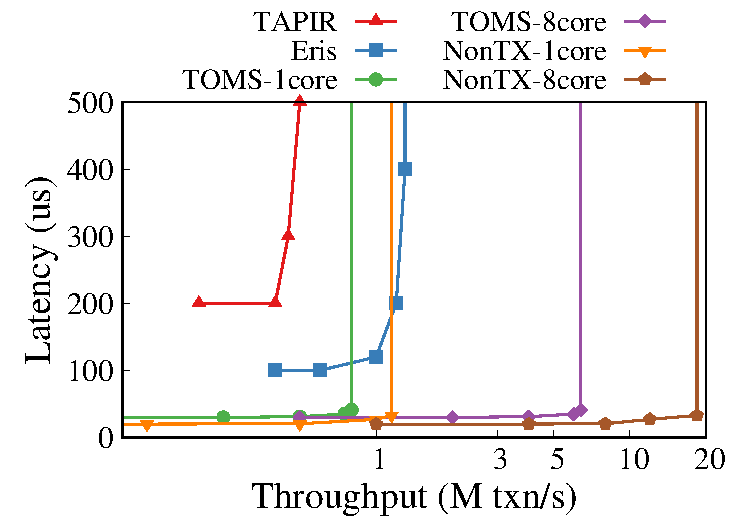
\includegraphics[width=.45\textwidth]{gnuplot/ycsb.pdf}
\caption{[Testbed] Throughput and latency of YCSB+T transactional key-value stores.}
\label{fig:ycsb}
\end{figure}


We use the same testbed setup as Sec.~\ref{sec:testbed}, and have one \sys client send transactions to 8 \sys servers as shards. We set the beacon interval to 10~$\mu$s.
Figure~\ref{fig:ycsb} shows the throughput and transaction latency of YCSB+T, where each operation accesses two randomly chosen objects.
TOMS achieves 6.4~M transactions per server (0.8~M transactions per core) with 40~$\mu$s latency. (We do not write logs to persistent storage.)
The throughput gap between TOMS and non-transactional system (NonTX) is mainly due to CPU processing of reordering messages.

\begin{figure}[t]
\centering
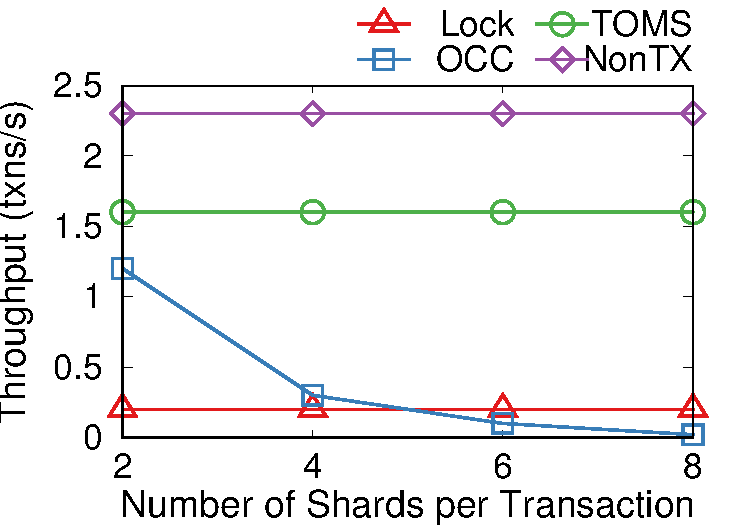
\includegraphics[width=.35\textwidth]{gnuplot/multishard.pdf}
\caption{[Testbed] Throughput of multiple shards per transaction.}
\label{fig:multishard}
\vspace{-10pt}
\end{figure}

Figure~\ref{fig:multishard} compares the throughput of TOMS, OCC, lock-based and non-transactional key-value stores.
Each transaction accesses 8 unique remote objects.
If the 8 objects are on two shards, OCC has 50\% chance of transaction abort, so the throughput is 50\% of non-transactional systems. When the objects are distributed on more shards, OCC has an exponentially higher chance of abort (Sec.~\ref{sec:toms}). The throughputs of other systems are unrelated to number of shards. \sys has 10x transaction throughput than lock-based systems, as well as OCC systems with more than 4 shards per transaction. The throughput of \sys is close to the theoretical bound of non-transactional system.



\begin{figure}[t]
\centering
	\subfloat[Throughput.\label{fig:loss-throughput}]
	{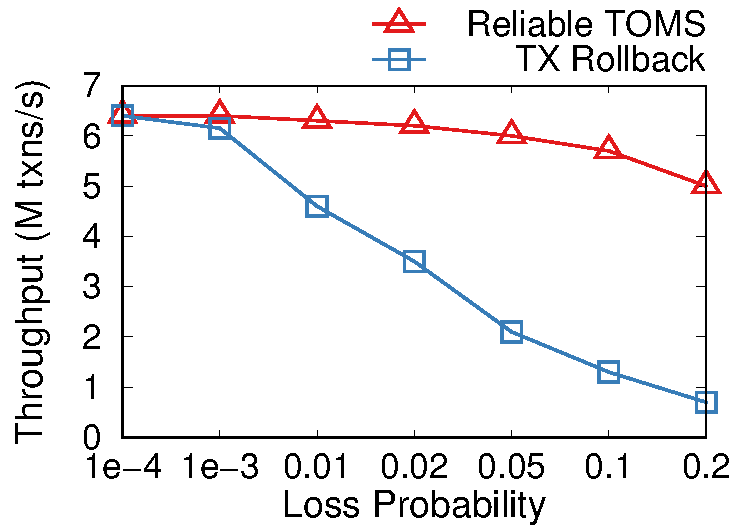
\includegraphics[width=.23\textwidth]{gnuplot/loss_tput.pdf}}
	\hspace{0.01\textwidth}
	\subfloat[Latency.\label{fig:loss-latency}]
	{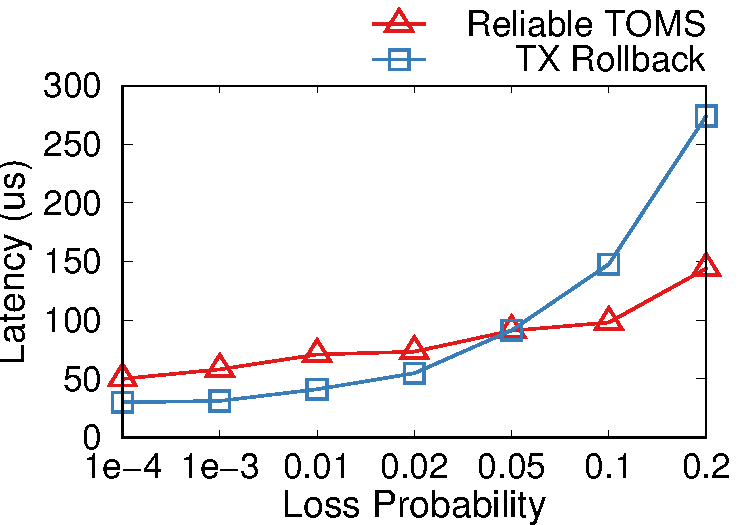
\includegraphics[width=.23\textwidth]{gnuplot/loss_latency.pdf}}
\caption{[Simulation] Comparison of reliable \sys and application-layer transaction rollback.}
\label{fig:ycsb-loss}
\end{figure}

Finally, we study the efficiency of our loss detection and recovery mechanism in Sec.~\ref{sec:lossy}.
Assume 1/10 of the transactions have conflicts, \textit{i.e.}, if a transaction is rollbacked, 1/10 of uncommitted transactions also need rollback.
Figure~\ref{fig:ycsb-loss} simulate the transaction throughput and latency under different loss ratios. With reliable \sys, packet loss is transparent to applications, and the transaction throughput is approximately the network goodput. If \sys does not handle packet loss, the transaction processing application needs to rollback all uncommitted transactions in conflict with the lost transaction, so a significant portion of CPU power and network bandwidth is wasted.

On the latency side, reliable \sys adds one RTT of latency to derive the ACK barrier. If any packet is lost, reliable \sys needs to wait for an additional RTT to retransmit the packet. When packet loss is rare, as in most data center networks, handling loss by applications provides lower latency. Under high packet loss probability, however, handling losses in \sys is better.

\iffalse
\begin{figure}[t]
\centering

\includegraphics[width=0.3\textwidth]{images/fixme.pdf}
\caption{[Testbed] Comparing YCSB+T throughput on inter-DC WAN.}
\vspace{-10pt}
\label{fig:ycsb-inter-dc}
\end{figure}

Figure~\ref{fig:ycsb-inter-dc} compares the throughput of cross-datacenter workload of TOMS and lock-based.
\fi

%\subsection{Multiple Round-Trip Transactions}

%TPC-C transaction benchmark

%Compare transaction throughput with Eris, TAPIR, DrTM+R (lock based), OCC and theoretical optimal (non-transactional)

%\subsection{Coordination-Free Causal Ordering}

%Our barrier timestamp is guaranteed to be lower than data timestamp, so if we send a message A after receiving a message B, A has higher timestamp than B. This can ensure ordering of events in a distributed system. For example, client A sends a command W to write database D, then sends a message to client B. When B receives the message from A, it sends command R to read database D. In our system, the database read command R is guaranteed to be processed after the write command W, so no additional synchronization is needed.